\section{Neutrino Interactions}
\label{sec:ew-interactions}

Left-handed neutrinos and right-handed antineutrinos can interact with quarks and leptons via the exchange of $Z^0$ (neutral-current) and $W^\pm$ (charged-current) bosons.
In practice, neutrinos are observed to either scatter off of electrons in reactions such as
\begin{equation}
    \nu_e + e^- \rightarrow \nu_e + e^-\;,
\end{equation}
or to interact with nucleons.
While the calculation of electron scattering is straight-forward from the electroweak Lagrangian, the scattering off nuclei is rather complicated and requires different approximations depending on the energy scale.
This chapter first describes the scattering processes that are most important for the purpose of neutrino detection at energies of \SI{>1}{\giga\eV}, where the total cross-section is dominated by interactions with nuclei.
It then briefly summarizes the process of coherent forward scattering that influences neutrino oscillations during propagation through bulk material.

\subsection{Weak interactions after symmetry-breaking}
Neutrino interactions with matter are described by Weak force interactions after electroweak symmetry-breaking described in \refsec{ew-symmetry-breaking}.
The Lagrangian for these interactions can be written as the sum of the neutral-current (NC) and charged-current (CC) interactions.
The NC part describes the exchange of neutral $Z^0$ bosons, which couples to all quarks and leptons except for right-handed neutrinos (if they exist).
For leptons, the NC Lagrangian reads
\begin{marginfigure}
\centering
\begin{subfigure}[t]{0.49\linewidth}
    \begin{tikzpicture}
        \begin{feynman}
        \def\flen{1.2}
        \def\boslen{1.2}
        \def\fangle{45}

        % in order to get the [dot] to work, we need to add the empty braces
        \vertex (v1) [dot] at (0, \boslen) {};
        \vertex (i1) at ($(v1) + (180-\fangle:\flen)$) {\(\pbar{\nu}_\mathcal{l}\)};
        \vertex (f1) at ($(v1) + (\fangle:\flen)$) {\(\pbar{\nu}_\mathcal{l}\)};
        \vertex (v2) at (0, 0);

        \diagram* {
          (i1) -- [fermion] (v1) -- [fermion] (f1),
          (v1) -- [boson, edge label=$Z^0$] (v2)
        };
        \end{feynman}
    \end{tikzpicture}
    \caption{neutrinos}
\end{subfigure}
\begin{subfigure}[t]{0.49\linewidth}
    \begin{tikzpicture}
        \begin{feynman}
        \def\flen{1.2}
        \def\boslen{1.2}
        \def\fangle{45}

        % in order to get the [dot] to work, we need to add the empty braces
        \vertex (v1) [dot] at (0, \boslen) {};
        \vertex (i1) at ($(v1) + (180-\fangle:\flen)$) {\(\mathcal{l}^\pm\)};
        \vertex (f1) at ($(v1) + (\fangle:\flen)$) {\(\mathcal{l}^\pm\)};
        \vertex (v2) at (0, 0);

        \diagram* {
          (i1) -- [fermion] (v1) -- [fermion] (f1),
          (v1) -- [boson, edge label=$Z^0$] (v2)
        };
        \end{feynman}
    \end{tikzpicture}
    \caption{charged leptons}
\end{subfigure}
\caption{Neutral-current lepton interaction vertices.}
\label{fig:nc-vertices}
\end{marginfigure}
\begin{equation}
  \mathcal{L}_\mathrm{NC,L} = -\frac{g}{2 c_W^2} \sum_{\mathcal{l}=e,\mu,\tau} (\bar{\nu}_{\mathcal{l}, L} \gamma^\mu \nu_{\mathcal{l}, L} + (2 s_W^2 - 1) \bar{e}_{\mathcal{l}, L} \gamma^\mu e_{\mathcal{l}, L} + 2s_w^2 \bar{e}_{\mathcal{l}, R} \gamma^\mu e_{\mathcal{l}, R}) Z^0_\mu\;, \label{eq:ew-nc-lagrangian}
\end{equation}
where $\nu$ denotes a neutrino field, $e$ a lepton field and the subscripts $L$ and $R$ denote left-handed and right-handed fields, respectively.
The coefficient $s_W$ ($c_W$) is the sine (cosine) of the Weinberg angle and $g$ is the coupling constant that determines the overall strength of the electroweak force.
This Lagrangian leads to the trilinear couplings shown in \reffig{nc-vertices}.
The couplings to quarks have the same form as those to the charged leptons up to a difference in coupling strength\sidenote{Quark mixing has no effect on neutral current interactions due to the GIM mechanism.}.
Neutral-current interactions conserve both the electric charge and lepton number, such that a neutral-current interaction of a neutrino will always produce a neutrino of the same flavor.

The charged-current (CC) part of the Weak Lagrangian in the flavor basis is
\begin{marginfigure}
\centering
\begin{subfigure}[t]{0.49\linewidth}
    \begin{tikzpicture}
        \begin{feynman}
        \def\flen{1.2}
        \def\boslen{1.2}
        \def\fangle{45}

        % in order to get the [dot] to work, we need to add the empty braces
        \vertex (v1) [dot] at (0, \boslen) {};
        \vertex (i1) at ($(v1) + (180-\fangle:\flen)$) {\(\bar{\nu}_\mathcal{l}\)};
        \vertex (f1) at ($(v1) + (\fangle:\flen)$) {\(\mathcal{l}^{+}\)};
        \vertex (v2) at (0, 0);

        \diagram* {
          (i1) -- [fermion] (v1) -- [fermion] (f1),
          (v1) -- [boson, edge label=$W^-$] (v2)
        };
        \end{feynman}
    \end{tikzpicture}
    \caption{$W^-$ vertex}
\end{subfigure}
\begin{subfigure}[t]{0.49\linewidth}
    \begin{tikzpicture}
    \begin{feynman}
        \def\flen{1.2}
        \def\boslen{1.2}
        \def\fangle{45}

        % in order to get the [dot] to work, we need to add the empty braces
        \vertex (v1) [dot] at (0, \boslen) {};
        \vertex (i1) at ($(v1) + (180-\fangle:\flen)$) {\(\nu_\mathcal{l}\)};
        \vertex (f1) at ($(v1) + (\fangle:\flen)$) {\(\mathcal{l}^{-}\)};
        \vertex (v2) at (0, 0);

        \diagram* {
          (i1) -- [fermion] (v1) -- [fermion] (f1),
          (v1) -- [boson, edge label=$W^+$] (v2)
        };
    \end{feynman}
    \end{tikzpicture}
    \caption{$W^+$ vertex}
\end{subfigure}
\caption{Charged-current lepton interaction vertices.}
\label{fig:cc-vertices}
\end{marginfigure}
\begin{equation}
    \mathcal{L}_\mathrm{CC} = -\frac{g}{\sqrt{2}} \sum_{\mathcal{l}=e,\mu,\tau} \bar{\nu}_{\mathcal{l},L} \gamma^\mu e_{\mathcal{l},L} W^+_\mu + \bar{e}_{\mathcal{l},L} \gamma^\mu \nu_{\mathcal{l},L} W^-_\mu\;\mathrm{+h.c.}\;.\label{eq:ew-cc-lagrangian}
\end{equation}
In contrast to neutral current interactions, the charged current interactions couple exclusively to left-handed fields\sidenote{The left-handed fields in the flavor basis are superpositions of mass eigenstates that may contain a (charge-conjugated) right-handed Majorana component as described in \refsec{neutrino-masses}}.
The associated lepton interaction vertices are shown in \reffig{cc-vertices}.

The weak CC interactions with quarks are affected by quark mixing as a result of their mass generation via the Higgs mechanism.
After electroweak symmetry breaking, the mass eigenstates and the flavor eigenstates of quarks are not identical but are instead mixed with a unitary matrix, $V$, that is also called the Cabbibo-Kobayashi-Maskawa (CKM) matrix.
In the basis of mass eigenstates, the Lagrangian for weak CC interactions with quarks is
\begin{equation}
    \mathcal{L}_\mathrm{CC,Q} = \frac{g}{\sqrt{2}} \sum_{\alpha=1}^3 \sum_{\beta=1}^3
    \bar{u}_{\alpha,L}\gamma^\mu V_{\alpha \beta} d_{\beta,L} W_\mu^+
     + \bar{d}_{\alpha,L}\gamma^\mu V_{\beta \alpha}^* u_{\beta,L} W_\mu^-
    \;\mathrm{+h.c.}\;,
\end{equation}
where the indices $\alpha$ and $\beta$ run over the generations.

\subsection{Neutrino-Lepton Scattering}
The simplest process to consider is that of a neutrino scattering off of a single lepton, such as
\begin{equation}
    \nu_\mu + e^- \rightarrow \mu^- + \nu_e
\end{equation}
via the exchange of a $W^+$ boson.
The Feynam diagram for this process is shown in \reffig{feynman-nue-scatter}.
To calculate the kinematics of this process, it is useful to define variables that are invariant under Lorentz transformations
\begin{equation}
\begin{aligned}
    s &= (p_\nu + p_e)^2 \\
    Q^2 &= (p_\nu - k_\nu)^2 \\
    y &= \frac{p_e \cdot q}{p_e \cdot p_\nu}\;,
\end{aligned}\label{eq:kinematic-quantities}
\end{equation}
where $s$ is the center of mass energy, $Q^2$ is the 4-momentum transfer, and $y$ is the inelasticity.
The inelasticity in the laboratory frame is the fraction of the energy carried by the outgoing lepton.
\begin{marginfigure}
\begin{tikzpicture}
\begin{feynman}
    \def\flen{2}
    \def\boslen{1.5}
    \def\fangle{20}

    % in order to get the [dot] to work, we need to add the empty braces
    \vertex (v1) [dot] at (0, \boslen) {};
    \vertex (i1) at ($(v1) + (180-\fangle:\flen)$) {$\nu_e$};
    \vertex (f1) at ($(v1) + (\fangle:\flen)$) {$e^-$};

    \vertex (v2) [dot] at (0, 0) {};
    \vertex (i2) at ($(v2) + (\fangle-180:\flen)$) {$e^-$};
    \vertex (f2) at ($(v2) + (-\fangle:\flen)$) {$\nu_e$};

    \diagram*{
        (i1) [particle=$\nu_\mu$]-- [fermion, momentum=$p_\nu$] (v1) -- [fermion, momentum=$k_\mu$] (f1) [particle=$\mu^-$],
        (v1) -- [boson, edge label'=$W^+$] (v2),
        (i2) [particle=$e^-$] -- [fermion, momentum'=$p_e$] (v2) -- [fermion, momentum'=$k_e$] (f2) [particle=$\nu_e$],
    };
\end{feynman}
\end{tikzpicture}
\caption{Feynman diagram for neutrino-electron scattering.\label{fig:feynman-nue-scatter}}
\end{marginfigure}
For a two-body collision between a neutrino with a negligibly small mass and a stationary target electron, the differential cross-section is
\begin{equation}
    % converted eq.
    \frac{\drm \sigma}{\drm y} = \frac{m_e E_\nu}{8\pi}\frac{|\mathcal{M}|^2}{(s-m_e^2)^2}\;,
\end{equation}
in which $\mathcal{M}$ is the matrix element of the interaction.
The matrix element can be calculated at tree level from the Feynman diagram in \reffig{feynman-nue-scatter} and the charged-current Lagrangian from \refeq{ew-cc-lagrangian}.
In the case that $Q^2 \ll m_W$ and that the energy is well above the electron production limit, the matrix element is
\begin{equation}
    \mathcal{M}_{CC} = -\frac{G_F}{\sqrt{2}}\left\{ [\bar{e}\gamma^\mu(1-\gamma^5)\nu_e][\bar{\nu}_e\gamma_\mu(1-\gamma^5)e] \right\}\;.
\end{equation}
Here, the constant $G_F$ is the fermi constant\cite{pdg}
\begin{equation}
    G_F = \frac{g^2}{2\sqrt{2}M_W^2} = \SI{1.1663788(6)e-5}{GeV^{-2}}\;.
\end{equation}
The integrated cross-section for this process is
\begin{equation}
    \sigma \simeq \frac{G^2_F s}{\pi}\;.
\end{equation}

\subsubsection{Particle-antiparticle scattering}
\label{sec:antineutrino-scattering}
In a reaction between a particle and an antiparticle, such as
\begin{equation}
    \bar{\nu}_\mu + e^- \rightarrow \mu^-  + \bar{\nu}_e\;,
\end{equation}
the different spin states introduce a preferred direction to the scattering process due to the conservation of angular momentum.
This can be seen easily when the reaction is illustrated in the center-of-mass frame as in \reffig{spin-config}.
The scattering process is kinematically suppressed by a factor of $(1 + \cos \theta^*)^2/4$, even though the matrix element for the reaction is the same as for particle-particle scattering.
\begin{figure}
\begin{subfigure}[t]{0.3\linewidth}
\begin{tikzpicture}
  \node (c) at (0,0)[shape=circle, fill=black, inner sep=1.5pt, outer sep=3pt] {};
  \draw [line width=0.2mm, arrows = {-Latex[scale=1]}] (180:1.2) node [anchor=east] {$e^-$} -- node [above, sloped] {$\Longrightarrow$} (c);
  \draw [line width=0.2mm, arrows = {-Latex[scale=1]}] (0:1.2) node [anchor=west] {$\bar{\nu}_\mu$}  -- node [above, sloped] {$\Longrightarrow$} (c);
\end{tikzpicture}
\caption{Initial state}
\end{subfigure}
\hfill
\begin{subfigure}[t]{0.3\linewidth}
\begin{tikzpicture}
  \node (c) at (0,0)[shape=circle, fill=black, inner sep=1.5pt, outer sep=3pt] {};
  \draw [line width=0.2mm, arrows = {Latex[scale=1]-}] (220:1.2) node [anchor=east] {$\bar{\nu}_e$} -- node [above, sloped] {$\Longrightarrow$} (c);
  \draw [line width=0.2mm, arrows = {Latex[scale=1]-}] (40:1.2) node [anchor=west] {$\mu^-$}  -- node [above, sloped] {$\Longrightarrow$} (c);
  \draw (0,0) -- node [near end, anchor=south] {$\theta^*$} (0.95,0) arc (0:40:0.95);
\end{tikzpicture}
\caption{Final state with small angle}
\end{subfigure}
\hfill
\begin{subfigure}[t]{0.3\linewidth}
\begin{tikzpicture}
 \node (c) at (0,0)[shape=circle, fill=black, inner sep=1.5pt, outer sep=3pt] {};
 \draw [line width=0.2mm, arrows = {Latex[scale=1]-}] (300:1.2) node [anchor=north] {$\bar{\nu}_e$} -- node [below, sloped] {$\Longleftarrow$} (c);
 \draw [line width=0.2mm, arrows = {Latex[scale=1]-}] (120:1.2) node [anchor=south] {$\mu^-$}  -- node [below, sloped] {$\Longleftarrow$} (c);
 \draw (0,0) -- (0.95,0) arc (0:120:0.95) node [midway, anchor=north east] {$\theta^*$};
\end{tikzpicture}
\caption{Final state with large angle}
\end{subfigure}
\caption{Spin configuration for particle-antiparticle interactions in the center-of-mass frame. Thin arrows ($\rightarrow$) indicate momentum, thick arrows ($\Rightarrow$) show angular momentum.\label{fig:spin-config}}
\end{figure}
The scattering angle in the center-of-mass frame, $\theta^*$, is related to the inelasticity by $y=(1-\cos\theta^*)/2$, and thus the cross-section picks up an additional factor of $(1 - y)^2$.
After integrating over $y$, the total cross-section is reduced by a factor of 3.
In practice, this spin suppression of large scattering angles means that antineutrinos produce on average more highly energetic secondary leptons, while the over-all cross-section is smaller than that of neutrinos.

\subsection{Neutrino Interactions with Nuclei}
\label{sec:neutrino-xsec}

At energies of \SI{>= 1}{\giga\eV}, the total cross-section of neutrinos is dominated by interactions with nuclei, while scattering off electrons can be effectively neglected.
There are three processes that each have different characteristic energy ranges.
The descriptions of these processes and their cross-sections largely follow those in \sidecite{Formaggio:2012aa}.

\subsubsection{Charged-current Quasi-elastic Scattering}
At energies below \SI{1}{GeV}, neutrinos do not resolve the inner structure of a nucleon and the scattering process can be described as an interaction with the nucleon as a whole as
\begin{equation}
\begin{aligned}
    \nu_\ell + n &\rightarrow p + \ell^-\;,\\
    \bar{\nu}_\ell + p &\rightarrow n + \ell^+\;.
\end{aligned}
\end{equation}
The differential cross-section for this process as a function of the neutrino energy $E_\nu$ is
\begin{equation}
    \frac{\drm\sigma}{\drm Q^2} = \frac{G_F^2 M^2 |V_{ud}|^2}{8\pi E^2_\nu}
    \left[
        A \pm \frac{s-u}{M^2}B + \frac{(s-u)^2}{M^4}C
    \right]\;,\label{eq:ccqe-xsec}
\end{equation}
in which $V$ is the CKM matrix, $G_F$ is the Fermi constant, $Q^2$ is the squared four-momentum transfer and $M$ is the nucleon mass.
The $\pm$ sign is positive for neutrinos and negative for antineutrinos.
The variables $s$ and $u$ are Mandelstam variables that are functions of the momentum transfer and the factors $A$, $B$ and $C$ are functions of the form factor of the nucleon.
In practice, these factors depend largely only on the vector ($F_1$ and $F_2$) and axial-vector ($F_A$) form factor, the latter of which is
\begin{equation}
    F_A(Q^2) = \frac{g_A}{\left(1 + \frac{Q^2}{(M_A^{CCQE})^2}\right)^2}\;,\label{eq:axial-mass-form-factor}
\end{equation}
where $M_A^{CCQE}$ is the \emph{axial mass}.
Since the vector form factors and the coupling constant $g_A$ are well constrained from electron scattering and nuclear beta decay, respectively, the only free parameter that must be constrained directly from measurements of the neutrino cross-sections\cite{Lyubushkin:2009aa} is the axial mass.

\subsubsection{Neutral-current Elastic Scattering}
Cross-sections of neutral-current interactions of the form
\begin{equation}
\begin{aligned}
    \nu p &\rightarrow \nu p \\
    \nu n &\rightarrow \nu n
\end{aligned}
\end{equation}
are described by an equation that has the same form as \refeq{ccqe-xsec}, albeit with different coupling constants, and their most important uncertainties can be parametrized with the same axial mass as in \refeq{axial-mass-form-factor}.
For this reason, experiments have usually measured the ratio between CC and NC interactions.

\subsubsection{Resonant Scattering}
At energies of a few GeV, neutrino scattering can produce excited states of the nucleus in reactions such as
\begin{equation}
\begin{aligned}
    \nu_\ell + N &\rightarrow \ell^- + X^*\;, \\
    \bar{\nu}_\ell + N &\rightarrow \ell^+  + X^*\;,
\end{aligned}
\end{equation}
where $X^*$ is the excited state.
The differential cross-section for these processes can be approximated with an expression like \refeq{ccqe-xsec}, with different form factors and an independent axial mass parameter, $M_A^{CCRES}$.
The large number of possible resonant states and the necessary nuclear corrections make the correct calculation of the cross-section in this energy regime particularly challenging.

\subsubsection{Deep Inelastic Scattering}
At energies \SI{>10}{GeV}, the scattering process begins to resolve the inner structure of nuclei and neutrinos can scatter off of single quarks via the exchange of a $W^\pm$ or $Z^0$ boson, breaking up the struck nucleon into a shower of hadrons.
For muon neutrinos, the possible DIS processes are
\begin{equation}
\begin{aligned}
    \nu_\mu +N &\rightarrow \mu^- X &\bar{\nu}_\mu N &\rightarrow \mu^+ +X \\
    \nu_\mu +N &\rightarrow \nu_\mu X &\bar{\nu}_\mu N &\rightarrow \bar{\nu}_\mu +X\;. \\
\end{aligned}
\end{equation}
The Feynman diagram of the charged-current process is shown in \reffig{dis-cc-numu-feynman}.
The struck quark initiates a hadronization process that can produce multiple mesons in the output shower $X$.
\begin{figure}
\begin{tikzpicture}
\begin{feynman}
    % quark interaction point
    \vertex (interq) [dot] at (0,0) {};
    % lepton interaction point
    \vertex (interl) [dot] at (0, 2.2) {};
    % in/out leptons
    \vertex (il) at (-3, 3) {$\nu_\mu$};
    \vertex (ol) at (3, 3) {$\mu^-$};
    % input quarks (nucleus)
    \vertex (nuc) [shape=circle, draw, inner sep=0.3cm, fill=gray!30] at (-3, -1) {$N$};
    % output quarks (shower)
    \vertex (x1) at (3, -0.5) {};
    \vertex[below=0.4cm of x1] (x2) {};
    \vertex[below=0.4cm of x2] (x3) {};
    \vertex (hadr) at ($(x2)!0.5!(x3) + (-2,0.2)$);
    \vertex[below=0.4cm of x3] (x4) {};
    \vertex[below=0.4cm of x4] (x5) {};


    \diagram*{
        (nuc.north east) -- [fermion, edge label'=$d$, momentum=$p_i$] (interq) -- [fermion, edge label'=$u$, momentum=$p_f$] (x1),
        (nuc.east) -- [fermion] (x4),
        (nuc.south east) -- [fermion] (x5),
        %(x2) -- [fermion] (hadr) -- [fermion] (x3),
        (interq) -- [boson, edge label=$W^+$] (interl),
        (il) -- [fermion, momentum=$p_\nu$] (interl) -- [fermion, momentum=$p_\mu$] (ol),
    };

    \draw [decoration={brace}, decorate]  (x1.north east) -- (x5.south east) node [pos=0.5, right] {$X$};
\end{feynman}
\end{tikzpicture}
\caption{Deep inelastic scattering of a muon neutrino in the quark-parton model.\label{fig:dis-cc-numu-feynman}}
\end{figure}
The kinematics of this reaction can be calculated using the same Lorentz-invariant quantities that are defined for neutrino-lepton scattering in \refeq{kinematic-quantities} and one additional variable,
\begin{equation}
    x\equiv \frac{Q^2}{p_N \cdot q} = \frac{Q^2}{(s-m_N^2)y}
\end{equation}
that is referred to as Bjorken-$x$.
In the lab frame, the inelasticity is the fraction of the energy of the initial neutrino that is converted into hadrons
\begin{equation}
    y_\mathrm{lab} = 1 -\frac{E_\mu}{E_\nu} = E_\mathrm{hadrons}/E_\nu\;.
\end{equation}
The conditions for deep inelastic scattering to occur are
\begin{equation}
\begin{aligned}
    Q^2 &\gg m_N^2 \\
    p_N \cdot q &\gg m_N^2 \\
    s &\gg m_N^2\;.
\end{aligned}
\end{equation}
Under these conditions, the differential cross-sections for DIS for neutrinos and antineutrinos scattering off of a nucleon are
\begin{equation}
\begin{aligned}
    \frac{\drm^2 \sigma_\mathrm{CC}^{\nu N}}{\drm x \drm y}
    &= 2x\sigma^0_\mathrm{CC} \left[
        \sum_{q=d,s} f_q^N(x) + (1 - y)^2\sum_{\bar{q}=\bar{u},\bar{c}} f_{\bar{q}}^N(x)
    \right] \\
    \frac{\drm^2 \sigma_\mathrm{CC}^{\bar{\nu} N}}{\drm x \drm y}
    &= 2x\sigma^0_\mathrm{CC} \left[
        \sum_{\bar{q}=\bar{d},\bar{s}} f_{\bar{q}}^N(x) + (1 - y)^2\sum_{q=u,c} f_q^N(x)
    \right]\;,
\end{aligned}\label{eq:ccdis-xsec}
\end{equation}
with
\begin{equation}
    \sigma_\mathrm{CC}^0 = \frac{G_F^2}{2\pi}s \left( 1 + \frac{Q^2}{m_W^2} \right)^{-2}\;.
\end{equation}
The functions $f_{\pbar{q}}^N(x)$ are the parton distribution functions for each type of quark inside a nucleus.
The factor of $(1 - y)^2$ for scattering processes that mix particles and antiparticles comes from conservation of angular momentum, as outlined earlier for neutrino-lepton scattering.
This kinematic suppression reduces the inclusive cross-section for antineutrinos by a factor of approximately two.
The cross-section for neutral-current interactions has the same form as \refeq{ccdis-xsec}, only that the mass $m_W$ is replaced by $m_Z$ and the sum runs over left-handed and right-handed quark states that each have different coupling constants.
\begin{figure*}
\begin{subfigure}[t]{0.45\linewidth}
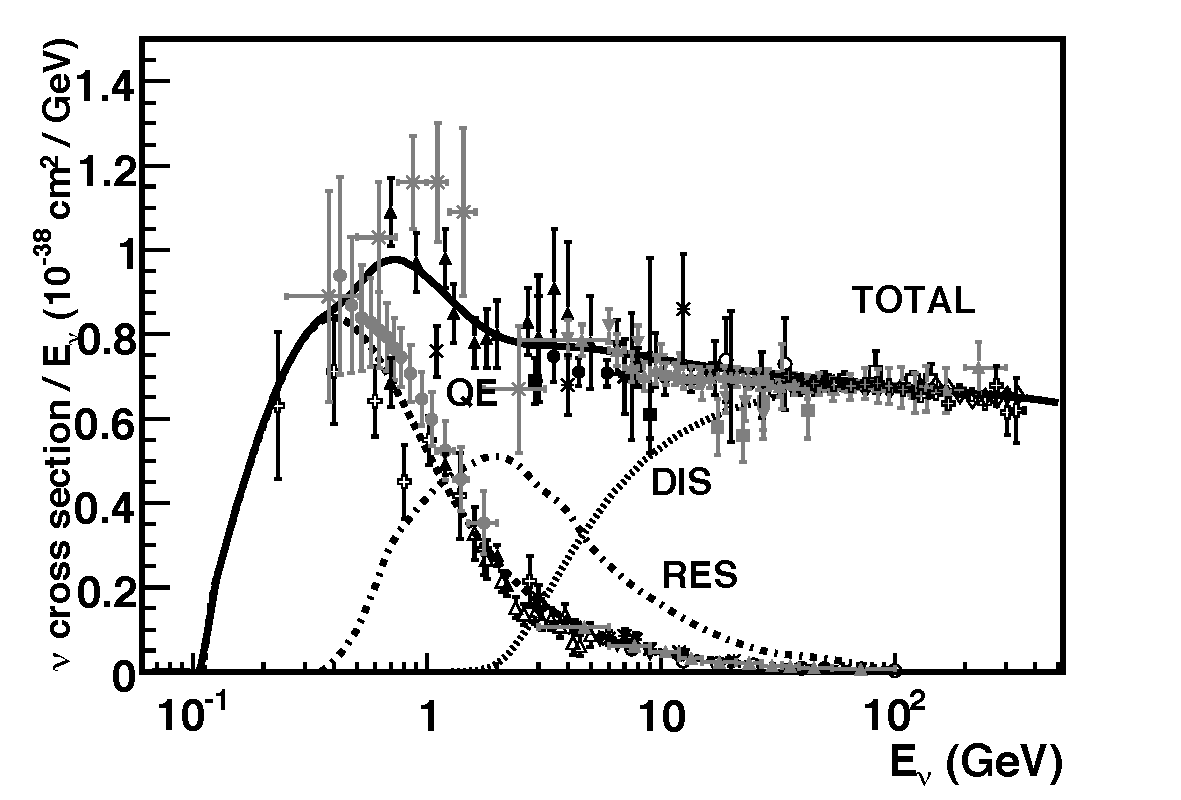
\includegraphics[width=\textwidth]{figures/theory/cc_inclusive_nu.pdf}
\caption{neutrinos}
\end{subfigure}
\begin{subfigure}[t]{0.45\linewidth}
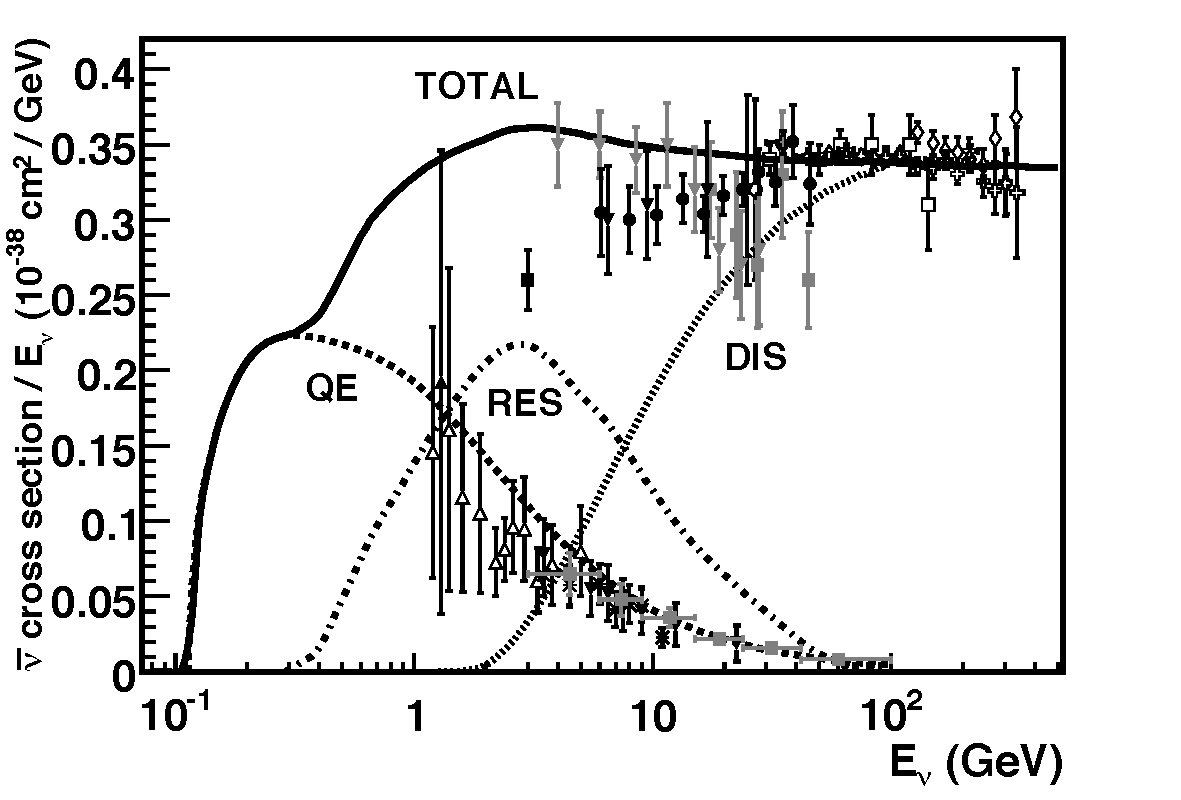
\includegraphics[width=\textwidth]{figures/theory/cc_inclusive_nubar.pdf}
\caption{antineutrinos}
\end{subfigure}
\caption{Inclusive cross sections for neutrinos and antineutrinos. Figure taken from \cite{Formaggio:2012aa}.}
\end{figure*}
